%************************************************
\section{Procedure} % (fold)
\label{sec:eval_procedure}
%************************************************
We have developed a web page the participants were able access, read through the introduction to get up to speed with the terminology and where they could find the scenarios and tasks to finish the evaluation, as well as the feedback forms to help them get back to us with answers. This documentation can be accessed live on the project's evaluation web page \footnote{\url{http://karolyszanto.ro/MastersThesis/evaluation/index.html}} or in raw format in the source code repository \footnote{\url{https://github.com/ksza/MasterThesis_Report/tree/master/evaluation_html}}.\\

Going through the introduction, the participants were first introduced to concepts of context-aware computing, followed by an introduction to the egocentric-interaction paradigm and the situative space model. In the last part of the introduction we have presented the goals of our work and the features of the EgoSim framework.\\

%************************************************
\subsection{Evaluation Tasks} % (fold)
%************************************************
Next, the participants were given three scenarios. The first step was the WarmUp task, meant to make the participant familiar with the simulator's concepts and ways of interacting with the environment. This step did not require any feedback. The WarmUp task is detailed in Appendix \ref{sec:eval_warmup_scenario}.\\

In the second scenario we have developed a simulation for an Assisted Living Facility where objects around the human agent are categorised according to the SSM. For this task the participants have evaluated the system from the simulation user's point of view. They had to test a ready made simulation with the EgoSim framework. The second task is detailed in Appendix \ref{sec:eval_alf_scenario}. In Figure \ref{fig:eval_alf_tryout} a participant is evaluating the Assisted Living Facility (ALF) simulation.\\
\begin{figure}[H]
	\centering
	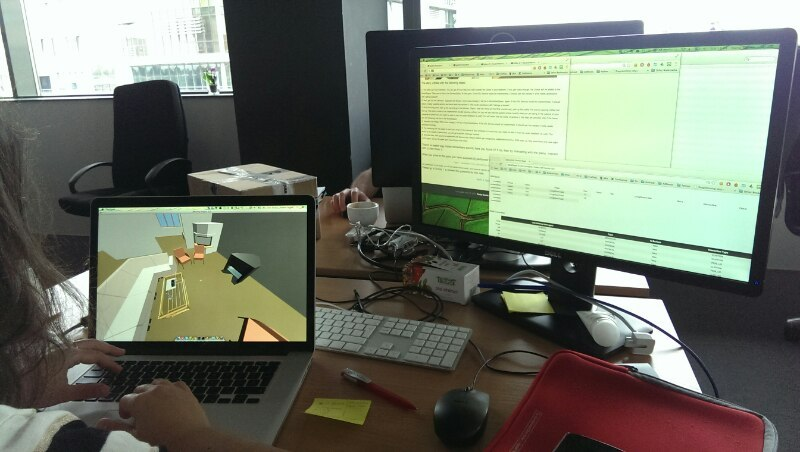
\includegraphics[width=\linewidth]{gfx/Chapter5/alf}
	\caption{A participant in our user-testing trying out the Assisted Living Facility Scenario}
	\label{fig:eval_alf_tryout}
\end{figure}

In the third scenario, the participants had to develop a new simulation using the EgoSim framework. The hypothetical problem they were given as part of this task is that families cannot make their homes secure enough for their children. Therefore, the participants were asked to imagine themselves being a system designer solving this problem using the EgoSim framework. This third task is detailed in Appendix \ref{sec:eval_childproof_scenario}. Setting up 3D models for EgoSim is done in third party software, therefore it is out of scope for its evaluation. We have provided all the 3D models needed by the participants to finalize the tasks. In Figure \ref{fig:eval_childproof_tryout} a participant is using EgoSim to build the Childproof simulation.\\
\begin{figure}[H]
	\centering
	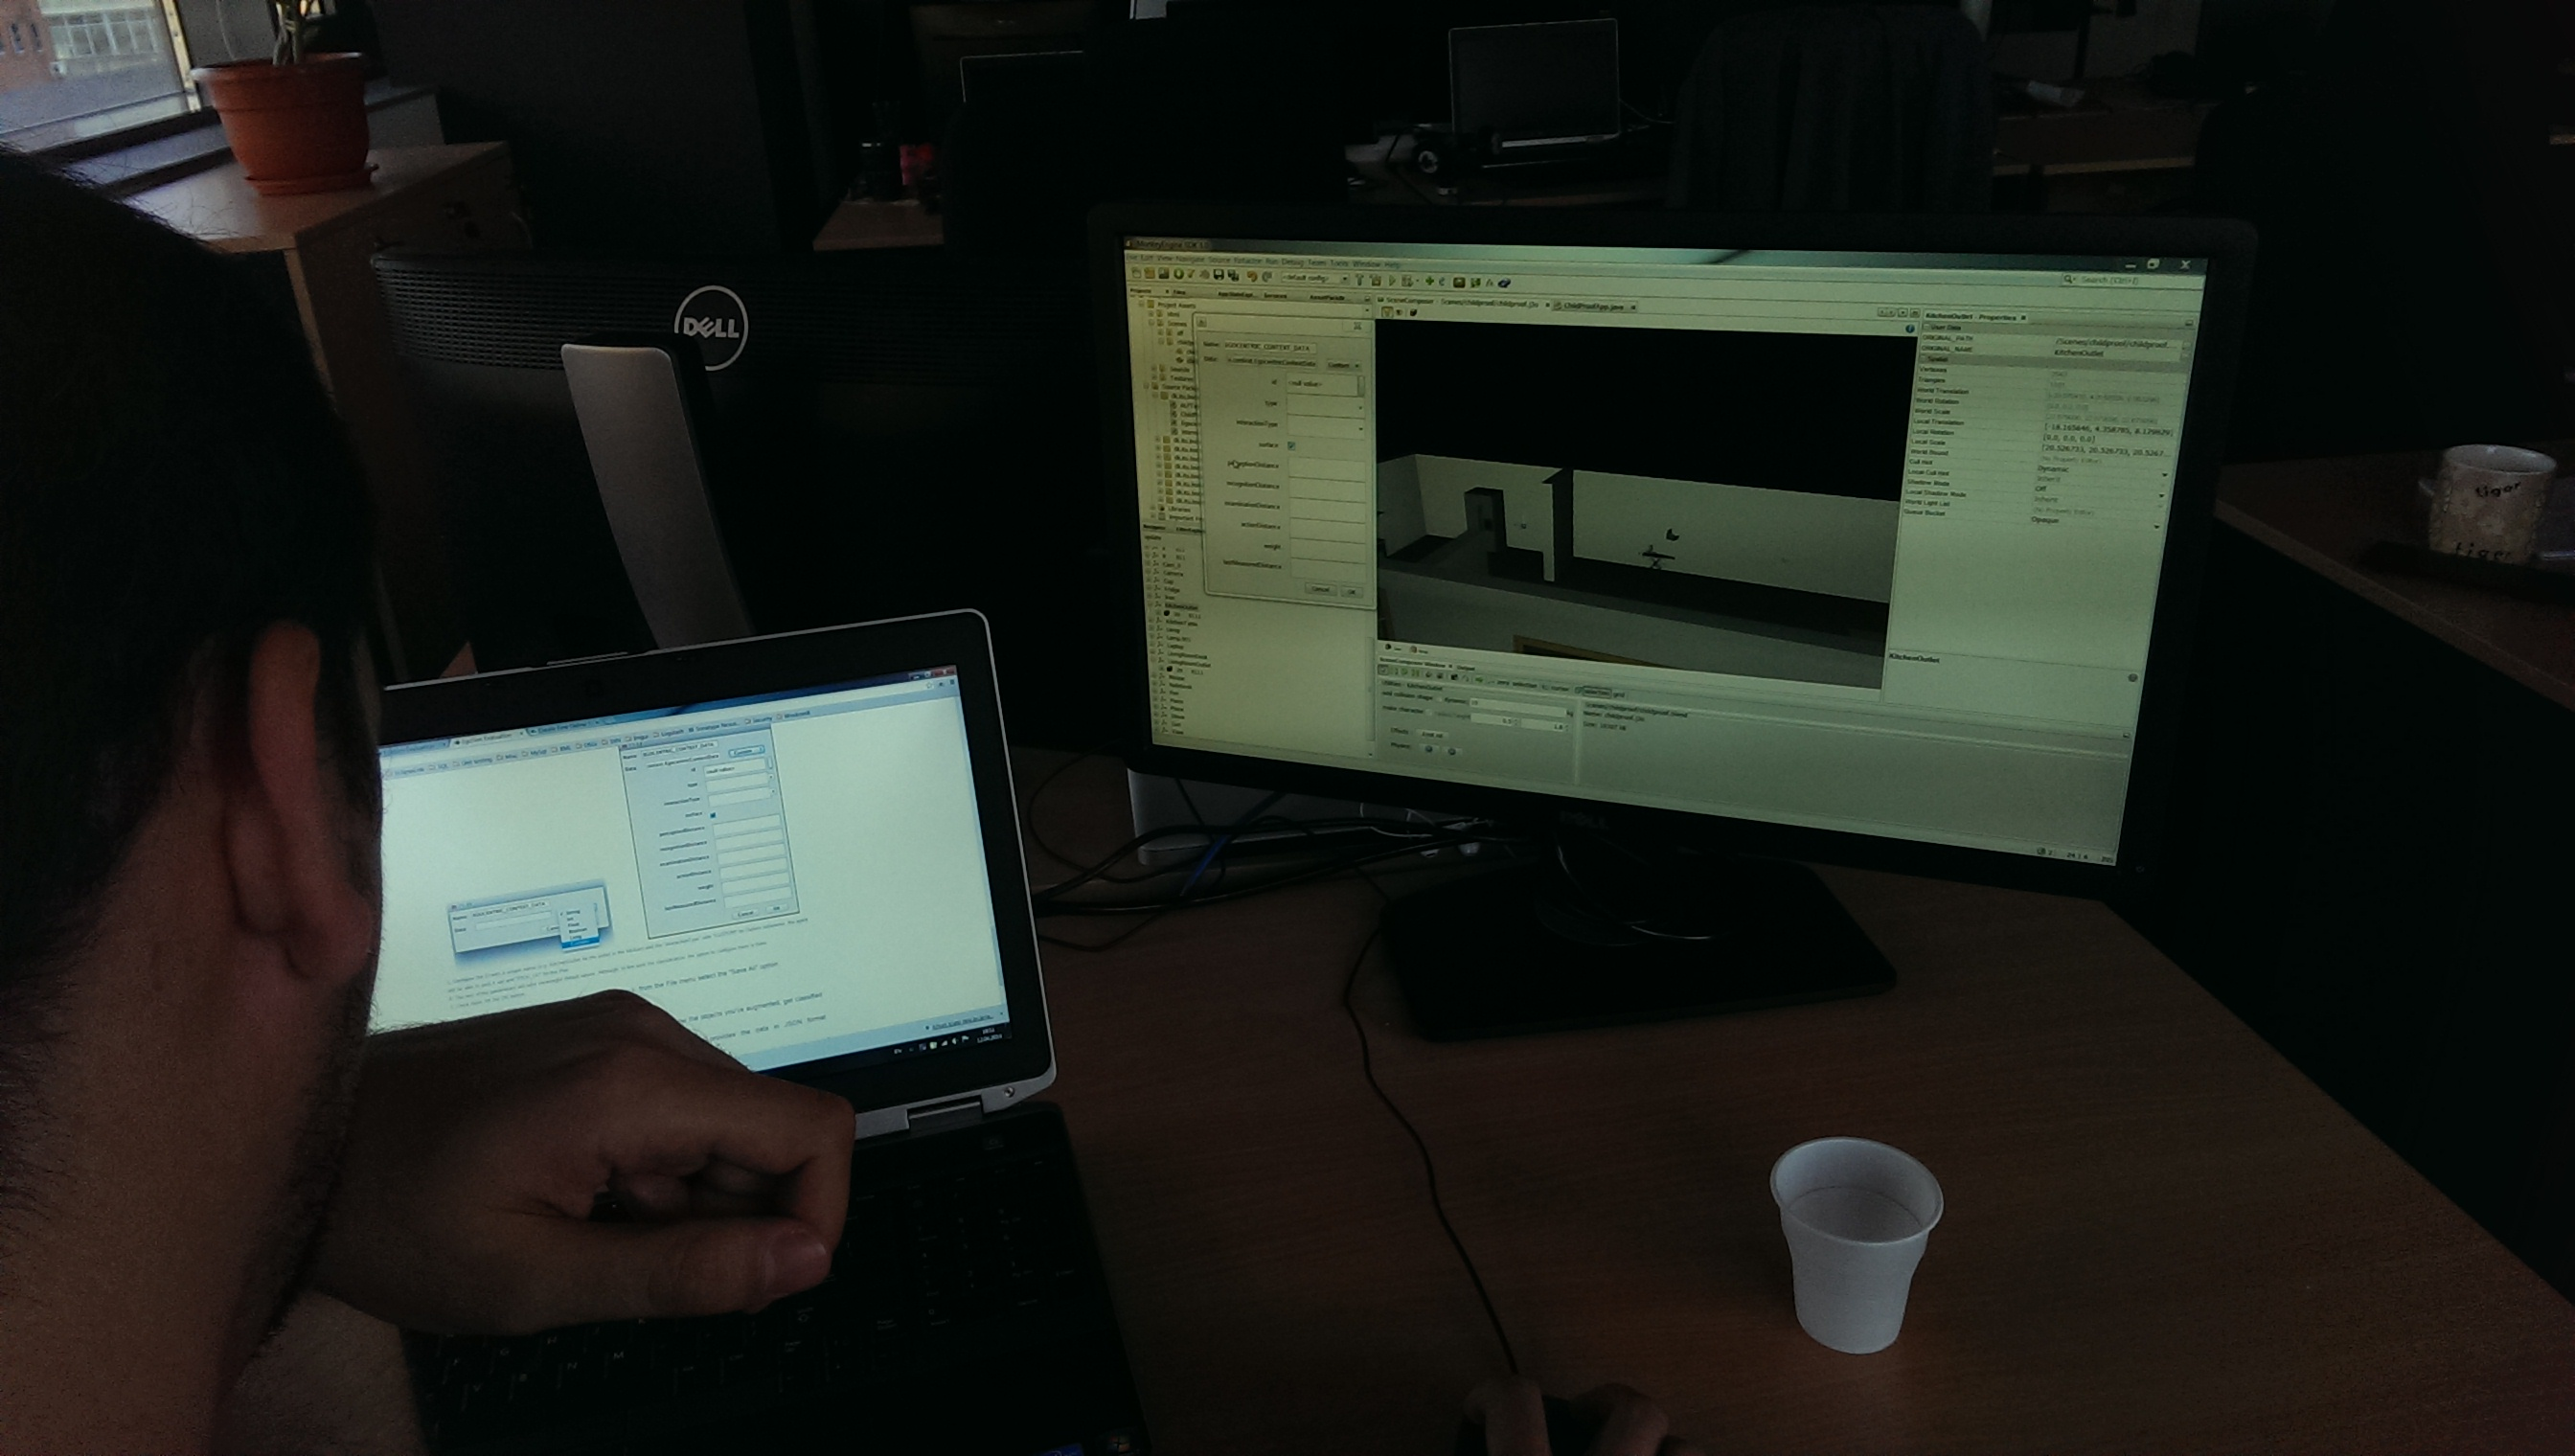
\includegraphics[width=\linewidth]{gfx/Chapter5/childproof}
	\caption{A participant in our user-testing building the simulation for the Childproof scenario}
	\label{fig:eval_childproof_tryout}
\end{figure}

Except for the warmup task, the participants were asked to fill in the feedback forms provided at the end of each evaluation scenario. The forms resemble a semi-structured interview which include questions regarding the usefulness of the system, usability of the framework and of the resulting simulations. We have asked many open questions encouraging the participants to provide detailed feedback that came to their mind about various aspects of the system (software bugs they might have found, what they liked, what they didn't, etc).\\

%************************************************
\subsection{Feedback \& Discussion} % (fold)
%************************************************
We would have liked to do a comparative study where the participants would create similar simulations using one of the systems presented in the related work chapter \ref{ch:related_work}. However, those systems do not support some of the features our system making it impossible to implement a replica of the same simulation. Moreover, the systems in the related work do not provide classification of objects around the agent according to the SSM, which makes the results of a comparison between a simulation built with EgoSim and one of the systems in the related work irrelevant. We therefore proceed with a user-test of our system with no comparison to other methods.\\

In the feedback form we have asked the participants a series of questions. The first set of question was about aspects of simulations built with EgoSim, asked from the simulation user's perspective as enumerated in Appendix \ref{sec:res_alf_task}. The second set of question was about the framework itself asked from the perspective of a system designer, as enumerated in Appendix \ref{sec:res_childproof_task}.\\

For a complete assessment of the framework, we should have covered the third role as well, evaluating the system from a third party system's point of view. Normally, we would have asked the participants to build a piece of software which connects to our API and implements some business login on top of the retrieved data. Instead, to reduce the evaluation time, in the second set of questions we gathered feedback about the API from the participants. Moreover, in the last question the participants were asked to describe in plain words or pseudo-code language the business logic to solve a given problem using the SSM Sets available through the API.\\

The whole evaluation session, including reading the documentation and providing feedback, lasted between 90 and 120 minutes. Videos of running the three scenarios are available; see Appendix \ref{ch:videos}. Next, in Section \ref{sec:eval_discussion} we will discuss the results of the evaluation.\\
% section sec:eval_procedure (end)